\chapter{理论与技术支持}

本章将介绍领域驱动设计战略建模和战术建模相关概念,
为构建战术建模方法做理论支持;
还将介绍建模语言相关概念以及特定领域建模语言构建方法,
作为构建战术建模语言的参考;
最后,将介绍建模支持工具实现技术,
为实现支持工具做技术支撑。


\section{领域驱动设计}

领域驱动设计与传统的建模分析方法不同,领域驱动设计不再只关注业务数据,
而是从领域中的重要概念出发,将业务流程中关键对象提炼成领域模型与关键逻辑,
来解决复杂业务的本质问题。由于战术建模中的概念依赖于战略建模,
并存在于某个战略建模的限界上下文(Bounded Context)中,
所以战略建模是战术建模实施的支撑背景。
本节将从战略建模和战术建模两个层次进行介绍,
重点关注战术建模中的重要概念。

\subsection{战略建模相关概念}


战略建模是从宏观角度对领域业务进行建模的建模方法,强调领域内的业务特性。
战略建模可以划分出业务的边界、组织团队结构以及系统架构,
为后续的战术建模划定限界上下文。
使用战略建模可以很好地进行微服务化拆分\cite{DBLP:conf/icsa/MersonY20}与系统拆分。
下面将对战略建模相关重要概念进行介绍。


\textbf{通用语言(Ubiquitous Language)}

通用语言是Eric Evans在《领域驱动设计:软件核心复杂性应对之道》\cite{DBLP:books/daglib/0013521}
中提出的术语,用于开发人员和用户建立通用、无歧义的语言。
该语言的基础是软件设计中的领域模型,应严格按照领域模型进行定义,保证其严谨性。
本文提出的战术建模语言及支持工具都使用通用语言进行表达。

\textbf{子域(Subdomain)}

领域可以进一步划分为核心域(Core Domain)、通用域(General Domain)和支撑域(Support Domain)。
每一个子域对应更小的问题域或业务范围,根据其自身的功能属性进行不同划分。

核心域决定业务的核心竞争力,是最重要的子域,包含主要的业务流程。
通用域是被其他多个子域共同使用的部分,没有定制化需求,包含通用功能。
支撑域最关注业务,对应某个业务中的重要部分,具有业务特定性,在不同企业业务中不通用,但必不可少。
本文提出的战术建模支持方法目的在于解决某个子域的建模问题。

\textbf{限界上下文(Bounded Context)}

限界上下文是一种概念性边界,限定了领域模型的工作范围。每一个模型概念和其中的
属性与操作,在它所属的边界之内,都有特定的含义,通过之前约定的通用语言,
参与建模的团队成员应该可以明确领域模型的具体含义。
对于系统架构来说,限界上下文还确定了应用边界和技术边界,提供了解决特定领域问题的
建模明确边界,同时也充当了问题空间与解空间之间的桥梁。
本文提出的战术建模支持方法工作范围在某个限界上下文之内,
可以聚焦于特定的业务领域,使建模中的交流成本变低。

\textbf{上下文映射(Context Map)}

上下文映射在项目团队中共享,并确保被每个团队成员理解。通过上下文映射,可以从宏观上
看到每个上下文之间的关系,能够更好地指导后续的程序设计。
上下文映射不拘泥于任何形式的文档,
重点在于帮助团队成员理解不同上下文之间的关系。
在不同限界上下文使用本文提出的建模支持方法进行战术建模后,可以通过上下文映射进行建模结果的交流。

\textbf{防腐层(Anti-Corruption Layer)}

防腐层可以根据领域模型为自身所在的限界上下文提供服务。
该层通过与另一个系统进行通信,几乎不需要对自身限界上下文进行任何修改。
防腐层需要在两个模型之间进行必要的双向转换\cite{DBLP:books/daglib/0013521}。
防腐层不仅防止内部代码被外部逻辑侵入,还在于分离不同的领域并确保它们在将来保持分离。
通过防腐层可以在战术建模支持方法中体现战略建模的底层基础作用。

战略建模首先需要确定通用语言,将要解决的领域问题划分为更细粒度的子域,
并通过划定限界上下文隔离不同领域模型的工作范围;
然后通过通用语言进行建模,借助上下文映射来理解不同限界上下文之间的关系,
最后还可以通过防腐层来与外部系统进行沟通。


\subsection{战术建模相关概念}

本小节将描述领域驱动设计战术建模的相关概念,战术建模是本文研究工作的重点内容,
战术建模支持方法基于战术建模相关概念提出。
战术建模是在特定的限界上下文中进行的更细粒度的建模,
可以用来管理领域模型的复杂性并确保领域模型中行为的准确性。
通用语言是将团队沟通与软件实现紧密联系到一起的一种基于模型的语言。
战术模式是战术建模中常用的表达业务问题的一种方式,
包含领域中的抽象概念、关系和约束规则,
并将领域模型和通用语言中的概念映射到实现技术中。
战术建模依赖通用语言和战术模式,
如图\ref{DDD}所示为模型驱动设计战术模式关系图,
展示了主要的战术模式与它们之间的关系,下面将对战术模式相关概念进行详细介绍并举例说明。

\begin{figure}[h] %figure环境,h默认参数是可以浮动,不是固定在当前位置。如果要不浮动,你就可以使用大写float宏包的H参数,固定图片在当前位置,禁止浮动。
    \centering %使图片居中显示
    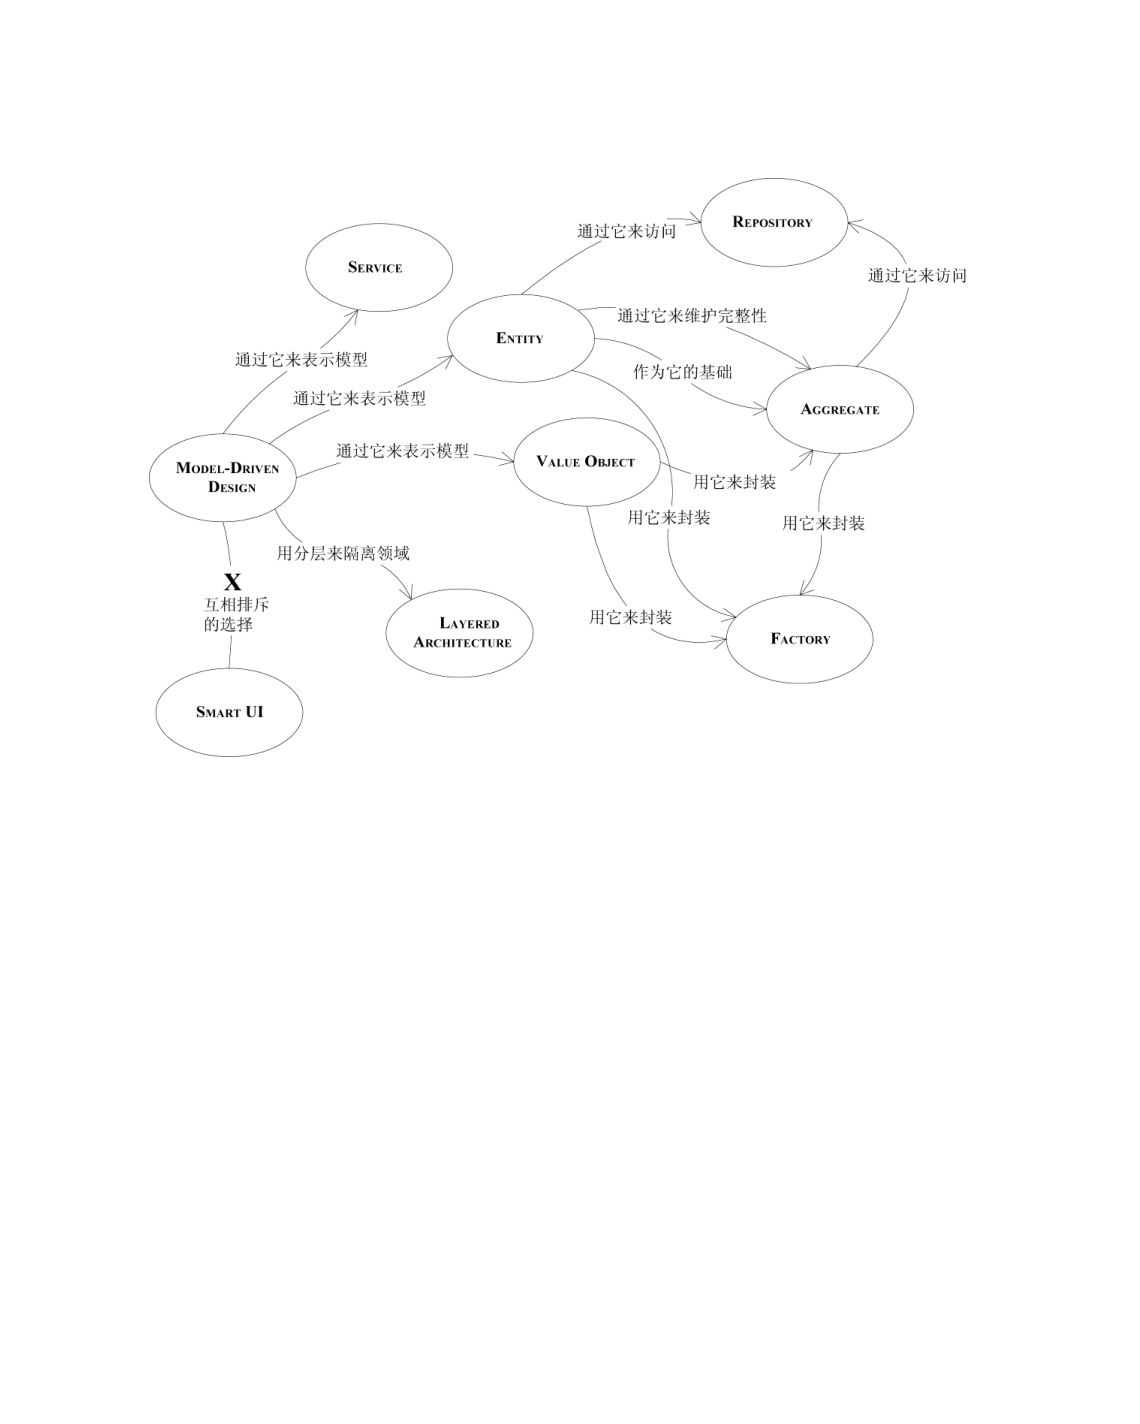
\includegraphics[width=0.8\textwidth]{FIGs/chapter2/DDD.pdf} %中括号中的参数是设置图片充满文档的大小,你也可以使用小数来缩小图片的尺寸。
    \caption{战术模式关系图\protect\footnotemark[1]} %caption是用来给图片加上图题的
    \label{DDD} %这是添加标签,方便在文章中引用图片。
\end{figure}%figure环境
\footnotetext[1]{图片来源于《领域驱动设计:软件核心复杂性应对之道》}

\textbf{实体(Entity)}

实体是一个由标识符定义的对象\cite{DBLP:books/daglib/0013521}。
当我们关注一个对象的个性特征,或者需要区分不同的对象时,我们使用实体这个概念,换句话说,
有必要将该对象与其他对象区别开来确保其个性特征时,我们希望将其建模成实体\cite{vernon2013implementing}。
例如,每辆汽车都通过车牌号与其他汽车进行区分,在这种条件下汽车应该被建模为实体。

\textbf{值对象(Value Object)}

值对象的作用是度量和描述事物,值对象可以很方便地进行创建、测试、使用、优化和维护。
值对象的使用比实体更加广泛,值对象一旦创建就不可变化,只可以进行替换,具有可比性\cite{vernon2013implementing}。
例如,一个人的家庭住址可以用来作为邮寄地址,当家庭住址改变时,可以直接将邮寄地址替换,
在这种条件下家庭住址应该被建模为值对象。

\textbf{领域服务(Domain Service)}

领域服务是一个独立接口,负责承担不属于实体或值对象职责的操作或转换过程。
领域服务可能关注一个显著的业务操作过程或领域对象的转换,
在单个原子操作中处理多个领域对象,并且命名要与通用语言保持一致\cite{vernon2013implementing}。
例如,保险公司在计算赔偿金额时需要进行复杂的计算流程,
而这种赔偿流程不是某个对象的职责,在这种条件下计算赔偿金额应该被建模为领域服务。

\textbf{领域事件(Domain Event)}

领域事件用来捕获发生在领域中的一些事情。领域事件记录了领域中已经发生的事情,无法改变。
需要维护业务一致性时,也需要用到领域事件,该事件往往是需要发布到外部系统(如外部限界上下文)的,
另外,领域事件还可以让远程依赖系统与本地系统保持一致\cite{vernon2013implementing}。
例如,在网购平台上订单已支付后,会触发商家发货等一系列流程,
在这种条件下订单已支付应该被建模为领域事件。

\textbf{聚合(Aggregate)}

聚合是一个将实体和值对象聚类到一致性边界内的容器。
聚合不仅仅是聚集了一些共享父类、密切关联的对象,更加重要的是其更关注内部的不变条件和整体的一致性边界\cite{vernon2013implementing}。
聚合根(Aggregate Root)是聚合用来标识自己的一个实体,需要追踪聚合变化时,就需要跟踪根实体,
根实体也是代表聚合与外界交互的对象。
例如,汽车是一种很复杂的机器,其中包含发动机、车轮、制动器等元件,
这些元件统一协同通信才组成了整个汽车,在这种条件下,
应该将这些元件组合到一起建模为聚合。

\textbf{资源库(Repository)}

资源库是一个用来存取领域对象的安全存储区域\cite{vernon2013implementing}。
可以通过资源库来安全地存储领域对象,并在需要时取出使用,资源库可以依据不同实现形式来
存取不同的领域对象。

\textbf{工厂(Factory)}

工厂是一种具有创建复杂对象和聚合职责的单独对象,该对象并不承担领域模型中的职责,
但是依然是领域驱动设计的一部分\cite{vernon2013implementing}。
创建复杂对象和聚合的逻辑经常封装在工厂中,与设计模式中的工厂相似,
但不应该为创建每个对象都提供一个工厂。
例如,组装汽车是一个复杂的过程,但最终产出仍然还是汽车,
在这种条件下,应该将创建汽车的工作建模成工厂。


\textbf{模块(Module)}

模块是一个命名的容器,用于存放内聚的类,
并可以对不在同一个模块的类解耦\cite{vernon2013implementing}。
主要应用在技术层面,如代码组织,构建目录与打包。
例如,汽车、飞机、轮船等交通工具在进行建模时,
可以统一放在交通工具模块中。

\section{建模语言}

战术建模与实现层次关联较强,甚至有些团队直接采用代码形式来进行建模,用代码来表达领域模型,
但这种方式不易于理解,在大型团队中无法很好地发挥领域模型的沟通作用。
建模语言是一种描述信息或者数据模型概念的语言,可以作为模型与实现之间沟通的桥梁,
UML就是一种统一建模语言。
构建元模型是实现建模语言的一种方式,
元模型可以作为交换和存储数据的介质或支持特定方法的语言,
UML也是通过元模型进行实现的建模语言。
通过对象约束语言对UML元模型的额外约束,
可以构建一种特定领域建模语言。
战术建模这一特定领域长期以来缺少标准、规范的建模语言来对建模过程进行规范化和约束,
随着战术建模应用越来越广泛,需要强大且合适的建模语言来进行支撑。

元模型(Metamodel)是描述模型的模型,在软件工程中使用模型来作为表达方式越来越普遍。
模型的建立背后应该对应着一个元模型,模型是真实世界中现象的抽象,
元模型是关注模型本身属性的一种抽象,所以可以把一个元模型看做对模型的抽象。
元模型可以充当交换或存储语义数据的中间介质,
可以作为支持特定方法或过程的语言,还可以作为扩展现有信息额外含义的语义语言\cite{emerson2006techniques}。
任何模型都应该服从其元模型的定义。
目前模型驱动工程(Model Driven Engineering,MDE)最活跃的分支是
Object Management Group(OMG)\footnotemark[2]\footnotetext[2]{OMG组织官网:https://www.omg.org/}
提出的模型驱动架构(Model Driven Architecture,MDA)解决方案\cite{soley2000model}。
该解决方案描述了被称为元对象机制(Meta-Object Facility,MOF)的元模型结构。
本文将采用元模型的方式来定义战术建模模型,战术建模语言也将以元模型为基础,
元模型是战术建模支持方法中建模语言的组成元素。


面向对象建模方法是一种依靠现实生活中常用思维来认识、理解和描述客观事物的建模方法,
强调最终建模的对象之间反映现实中的固有问题和关系。
面向对象分析与设计方法的发展在80年代末90年代初出现了一个高潮,由此出现了许多面向对象的建模方法。
其中具有代表性的如Yourdan等人\cite{coad1991object}提出的面向对象分析(Object-Oriented Analysis,OOA)方法,
Jacobson等人\cite{jacobson1995use}提出的面向对象软件工程(Object-Oriented Software Engineering,OOSE)方法等。
UML在此次高潮后,作为一种统一的建模语言产生。UML是一种建模语言,而不是方法,它不包含对过程的描述,
同时,UML也是OMG提出的典型元模型之一。

UML关注建模的普适性和可移植性,
直接使用UML进行战术建模粒度不够,
无法反映战术建模的一些模式及其规则和约束,会造成建模细节的损失。
特定领域建模语言(Domain Specific Modeling Language)\cite{{frank2013domain}}
是一种专注于某个特定领域,结合了特定领域知识和概念的建模语言。
分析领域的建模人员不必从头开始构建这些概念,
可以直接使用具有特定领域知识和概念的建模语言来进行建模,
所以,特定领域建模语言更加适合作为战术建模的基础语言。
本文构建特定于领域驱动设计战术建模的建模语言,包含战术建模相关概念,
使用该建模语言进行建模与战术建模目的相符。
同时UML可以适配任何适用于自己项目类型的过程,
并记录最终的分析和设计结果\cite{王文玲1999uml}。
因此,可以使用UML来作为建模结果的描述语言,
使建模结果具有通用性和普遍性,UML的profile扩展机制,
也提供了通过元模型(Metamodel)来确定构造型、约束和特定语义的方法,从而支持特定领域的建模过程。
针对于领域驱动设计战术建模,UML元类可以通过profile扩展机制,表示特定的模式,
如实体(Entity)、值对象(Value Object)等\cite{pahl2016microservices}。
本文将使用具有面向对象特征的UML profile扩展机制来作为元模型的实现方式,
既符合领域驱动设计的领域特征,又能扩充UML元模型构建新的建模语言。

对象约束语言是一种施加在指定模型元素上的约束语言。
对象约束语言最早是在1995年在IBM\footnotemark[3]\footnotetext[3]{IBM公司主页:https://www.ibm.com/}内部开发的,
1997年被集成到UML标准中,最初的作用是对UML表示法的补充,
OCL(Object Constraint Language)表达式能以附加在模型元素上的条件和限制来表现对该对象的约束,
克服了UML表示法甚至是任何图形表示法在系统详细设计时不够精确的局限性,
OCL充当了模型驱动工程(Model-Driven Engineering,MDE)技术的关键组成部分,
成为各种元模型查询,操作和制定规格要求的默认语言\cite{cabot2012object}。 
UML图表示法不够完善,无法规范化所有约束和属性,如果直接使用自然语言来表示,
会造成歧义,OCL也很好地填补了这一部分的空白。
本文提出的元模型经过OCL的附加约束,形成了完整的一套建模语言。

\section{特定领域建模语言构建方法}


本小节将介绍提出和验证特定领域建模语言的方法,
具体方法过程如图\ref{DSMLmethod}所示。
首先对特定的领域进行分析,得出基础理论知识;
然后根据知识设计元模型,进行细化;
将创建的元模型扩展为建模语言和工具,实现建模语言;
最后,对建模语言进行使用,验证效果\cite{sobernig2016extracting}。


\begin{figure}[h] %figure环境,h默认参数是可以浮动,不是固定在当前位置。如果要不浮动,你就可以使用大写float宏包的H参数,固定图片在当前位置,禁止浮动。
    \centering %使图片居中显示
    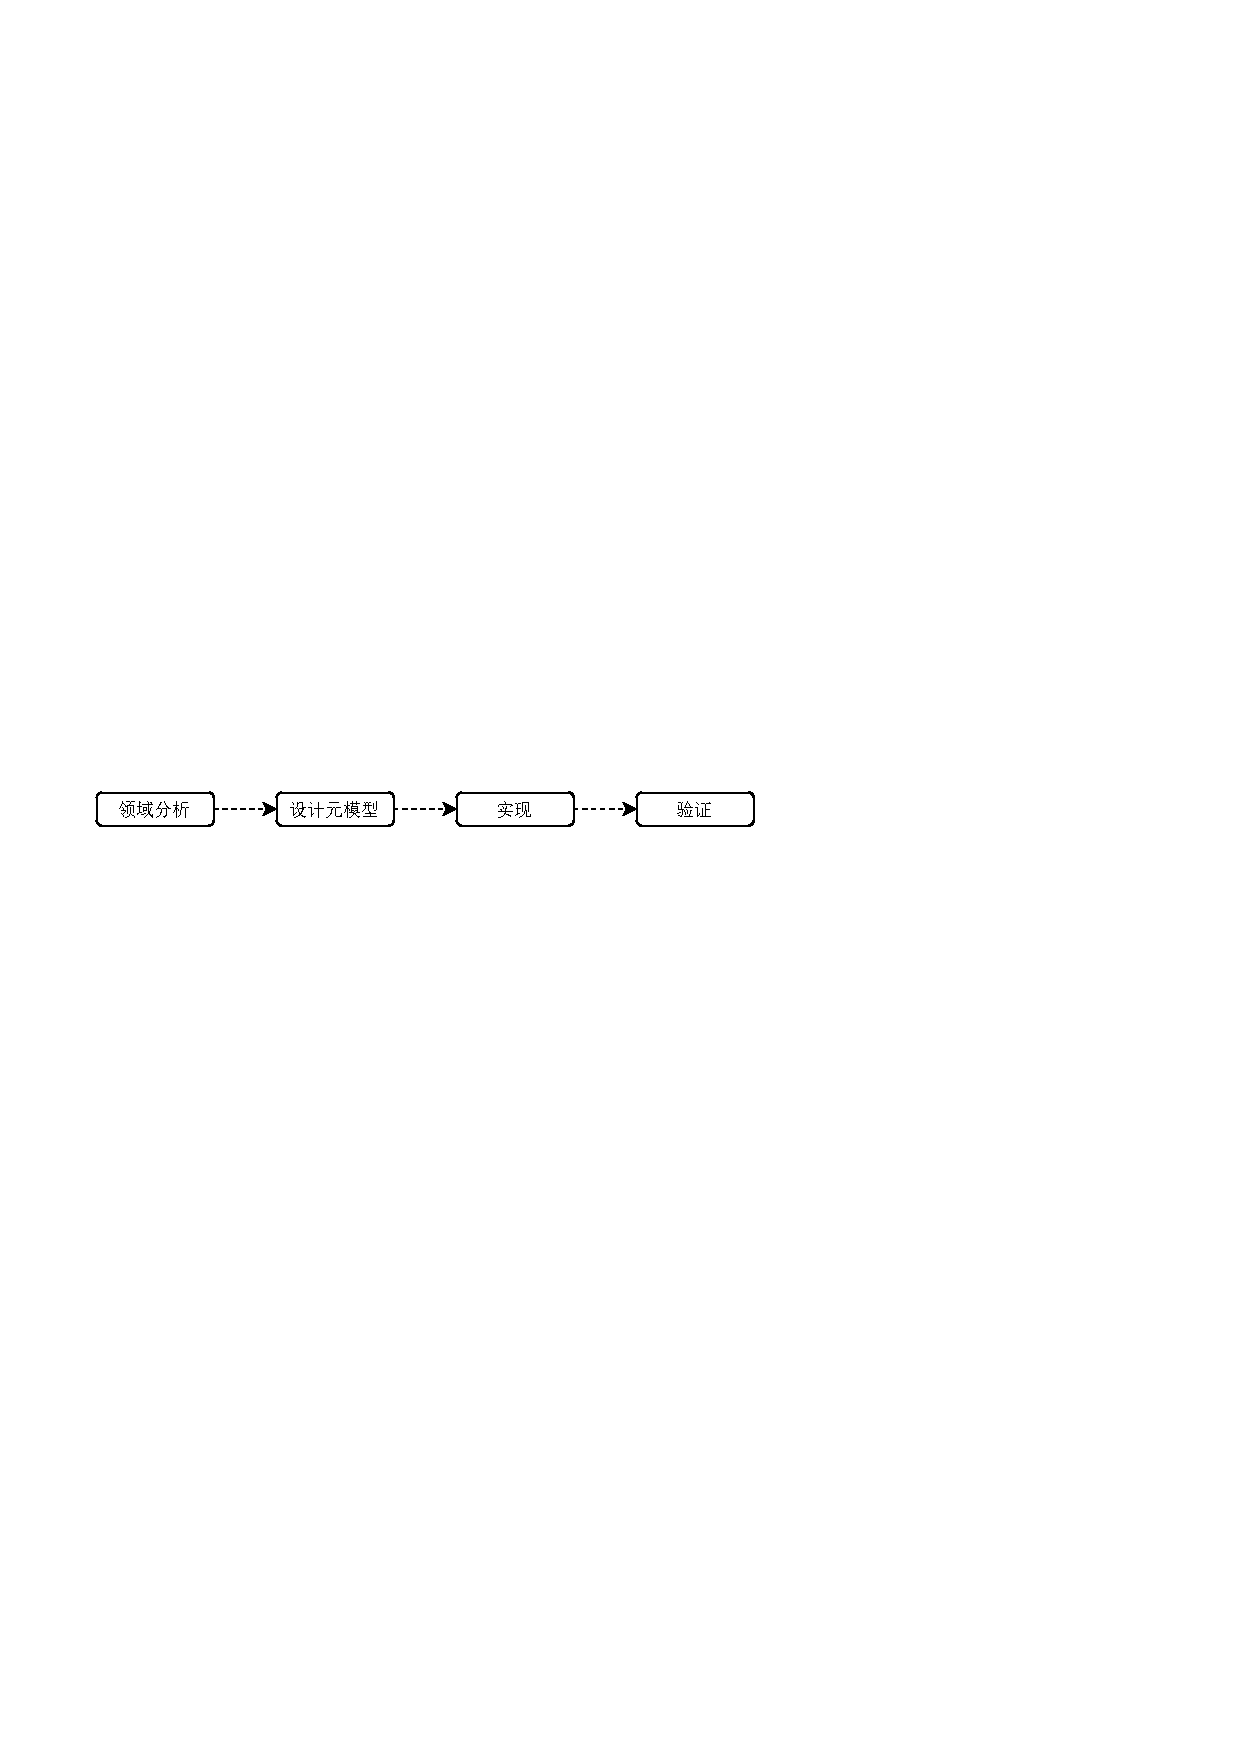
\includegraphics[width=0.8\textwidth]{FIGs/chapter3/DSMLmethod.pdf} %中括号中的参数是设置图片充满文档的大小,你也可以使用小数来缩小图片的尺寸。
    \caption{特定领域建模语言提出方法} %caption是用来给图片加上图题的
    \label{DSMLmethod} %这是添加标签,方便在文章中引用图片。
\end{figure}%figure环境

1)领域分析。这一阶段可以分为两种形式。第一种形式是由领域专家直接负责或参与,
由于领域专家拥有特定领域的丰富领域知识与实践经验,可以利用现有知识对特定领域重要概念进行提取,
抽象出一个初始的元模型,这种方法效率较高,适合于小范围领域,但最终建模语言质量依赖于领域专家的个人水平。
第二种形式是领域专家间接参与或不参与,这种形式需要通过阅读特定领域自然语言文献、对领域专家进行访谈或直接基于前人工作进行扩展,
得出基础理论知识或初始元模型,这种方法周期较长,适合比较成熟的领域。

2)设计元模型。这一阶段也可以在领域分析阶段直接完成。如果仅得到特定领域理论知识,需要使用理论知识构建元模型。
目前元模型的构建主要遵循的规则是元对象机制(Meta-Object Facility,MOF)定义的四层架构,UML也是MOF的一个实例\cite{bezivin2004search}。
如图\ref{MOF4}展示了MOF四层架构与UML类图之间的对应关系。M3元元模型层(Meta-Metamodel)包含了定义建模语言所需的元素,
作为整个框架的最高层,定义了最基本的元类(Metaclass),并且是自描述(Self-Descriptive)的;
M2元模型层(Metamodel)是M3元元模型的实例,定义了M1模型层需要使用的元素,如在类图中定义了“Operation”、“Class”、“Property”等元信息;
M1模型层(Model)是M2元模型层的具体实例,是用户根据M2元模型层定义所创建的具体模型实例,如类图中定义的具体类,以及该类包含的具体属性和操作;
M0实例层(Instance)是M1模型层的具体实例,是用户真正使用的实例对象,如根据类图创建的具体对象。

\begin{figure}[h] %figure环境,h默认参数是可以浮动,不是固定在当前位置。如果要不浮动,你就可以使用大写float宏包的H参数,固定图片在当前位置,禁止浮动。
    \centering %使图片居中显示
    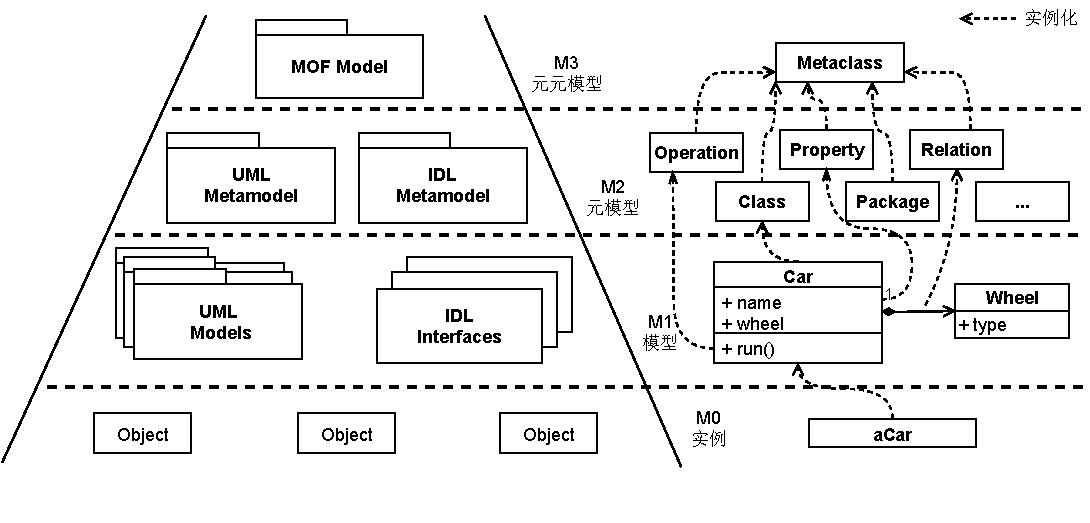
\includegraphics[width=0.8\textwidth]{FIGs/chapter3/MOF4.pdf} %中括号中的参数是设置图片充满文档的大小,你也可以使用小数来缩小图片的尺寸。
    \caption{MOF四层架构与UML类图\protect\footnotemark[4]} %caption是用来给图片加上图题的
    \label{MOF4} %这是添加标签,方便在文章中引用图片。
\end{figure}%figure环境
\footnotetext[4]{图片来源于OMG Unified Modeling Language (OMG UML), Superstructure}

在MOF四层架构与UML类图对应的基础上,进一步细化元模型设计,将重要领域概念与元模型元素对应起来。
UML中使用profile对M2元模型层进行扩展定义,提供了三种扩展方式:
构造型(Stereotype)是一个配置文件,可以通过构造型从现有的模型元素中派生出新的模型,
新的模型通常具有更适合特定领域的属性;
标记值(Tagged Values)用于扩展UML属性,可以在模型元素的规则中添加额外信息,
允许使用键值对的方式以字符串形式呈现,标记在模型元素下方,通常强调模型的版本控制,著作权等信息;
约束(Constraints)用于指定模型中必须始终满足的语义或条件,约束可以显示为字符串,
并包含在关联元素附近的方括号中。通常来限制模型中属性的取值范围。如图\ref{UMLprofileexample}
展示了UML profile扩展类图的一个实例。
构造型<<Machine>>表示图中Car类为扩展的机器类型,
标记值表示了该Car类的版本号,约束保证了该Car类的速度数值限制在0到300之间。

\begin{figure}[!htbp] %figure环境,h默认参数是可以浮动,不是固定在当前位置。如果要不浮动,你就可以使用大写float宏包的H参数,固定图片在当前位置,禁止浮动。
    \centering %使图片居中显示
    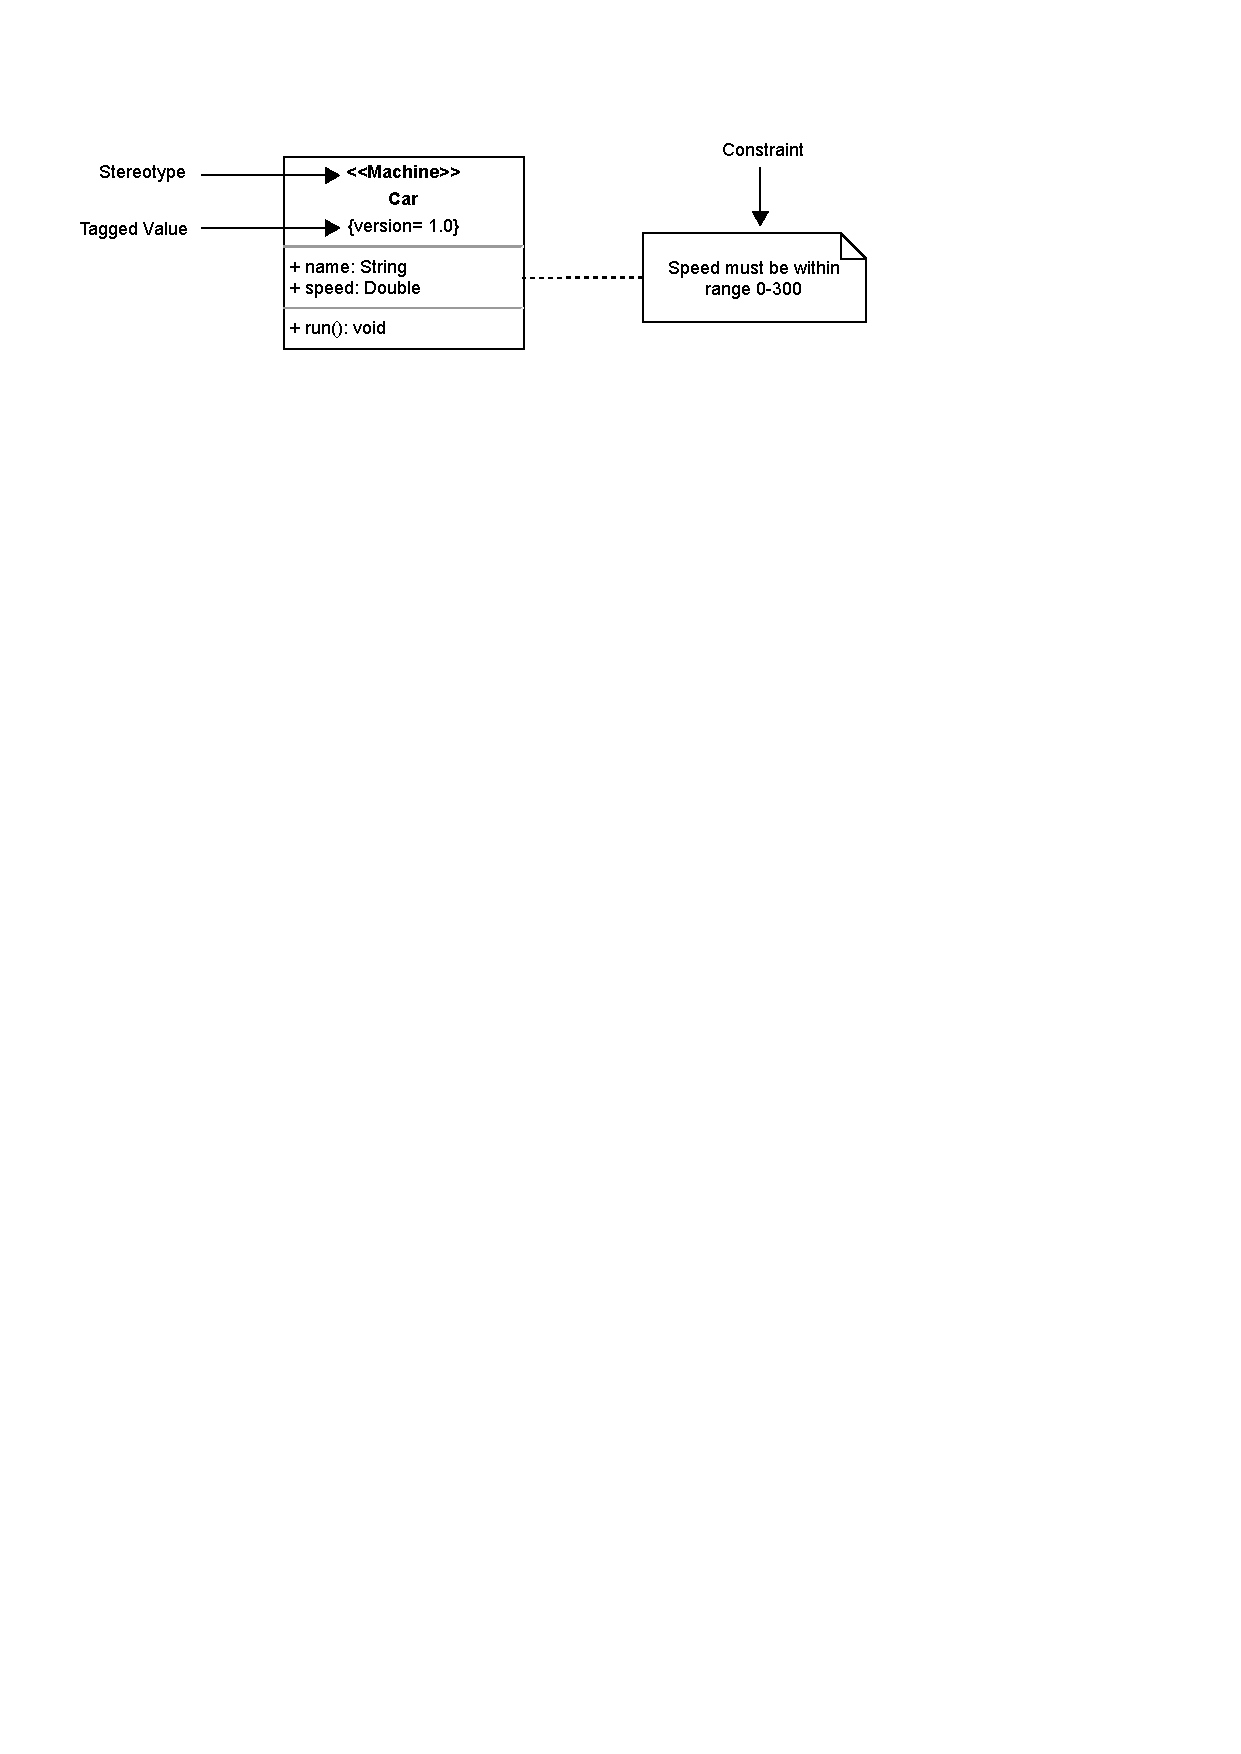
\includegraphics[width=0.8\textwidth]{FIGs/chapter3/UMLprofileexample.pdf} %中括号中的参数是设置图片充满文档的大小,你也可以使用小数来缩小图片的尺寸。
    \caption{UML profile扩展类图实例} %caption是用来给图片加上图题的
    \label{UMLprofileexample} %这是添加标签,方便在文章中引用图片。
\end{figure}%figure环境

3)实现。将设计完成的元模型结合理论知识运用到生产中,是这一阶段的主要任务。
建模工具的实施方式分为两种,如图\ref{2kindsmodeling}展示了两种不同实施工具的方式。
第一种方式通过扩展通用建模工具实施,这种方式依赖现有的支持通用建模语言的工具或平台,
将特定领域的建模语言配置文件导入,来支持新的建模语言。该方式有利于多种建模语言的集成,
但需要统一建模语言平台提供扩展功能。第二种方式通过建模工具生成器根据元模型生成相应的建模工具,
这种方式可以给用户提供一个独立的工具,有利于对建模工具的定制、修改和优化,
但添加额外功能困难, 依赖于工具生成器的成熟度\cite{刘辉2008元建模技术研究进展}。


\begin{figure}[!htbp] %figure环境,h默认参数是可以浮动,不是固定在当前位置。如果要不浮动,你就可以使用大写float宏包的H参数,固定图片在当前位置,禁止浮动。
    \centering %使图片居中显示
    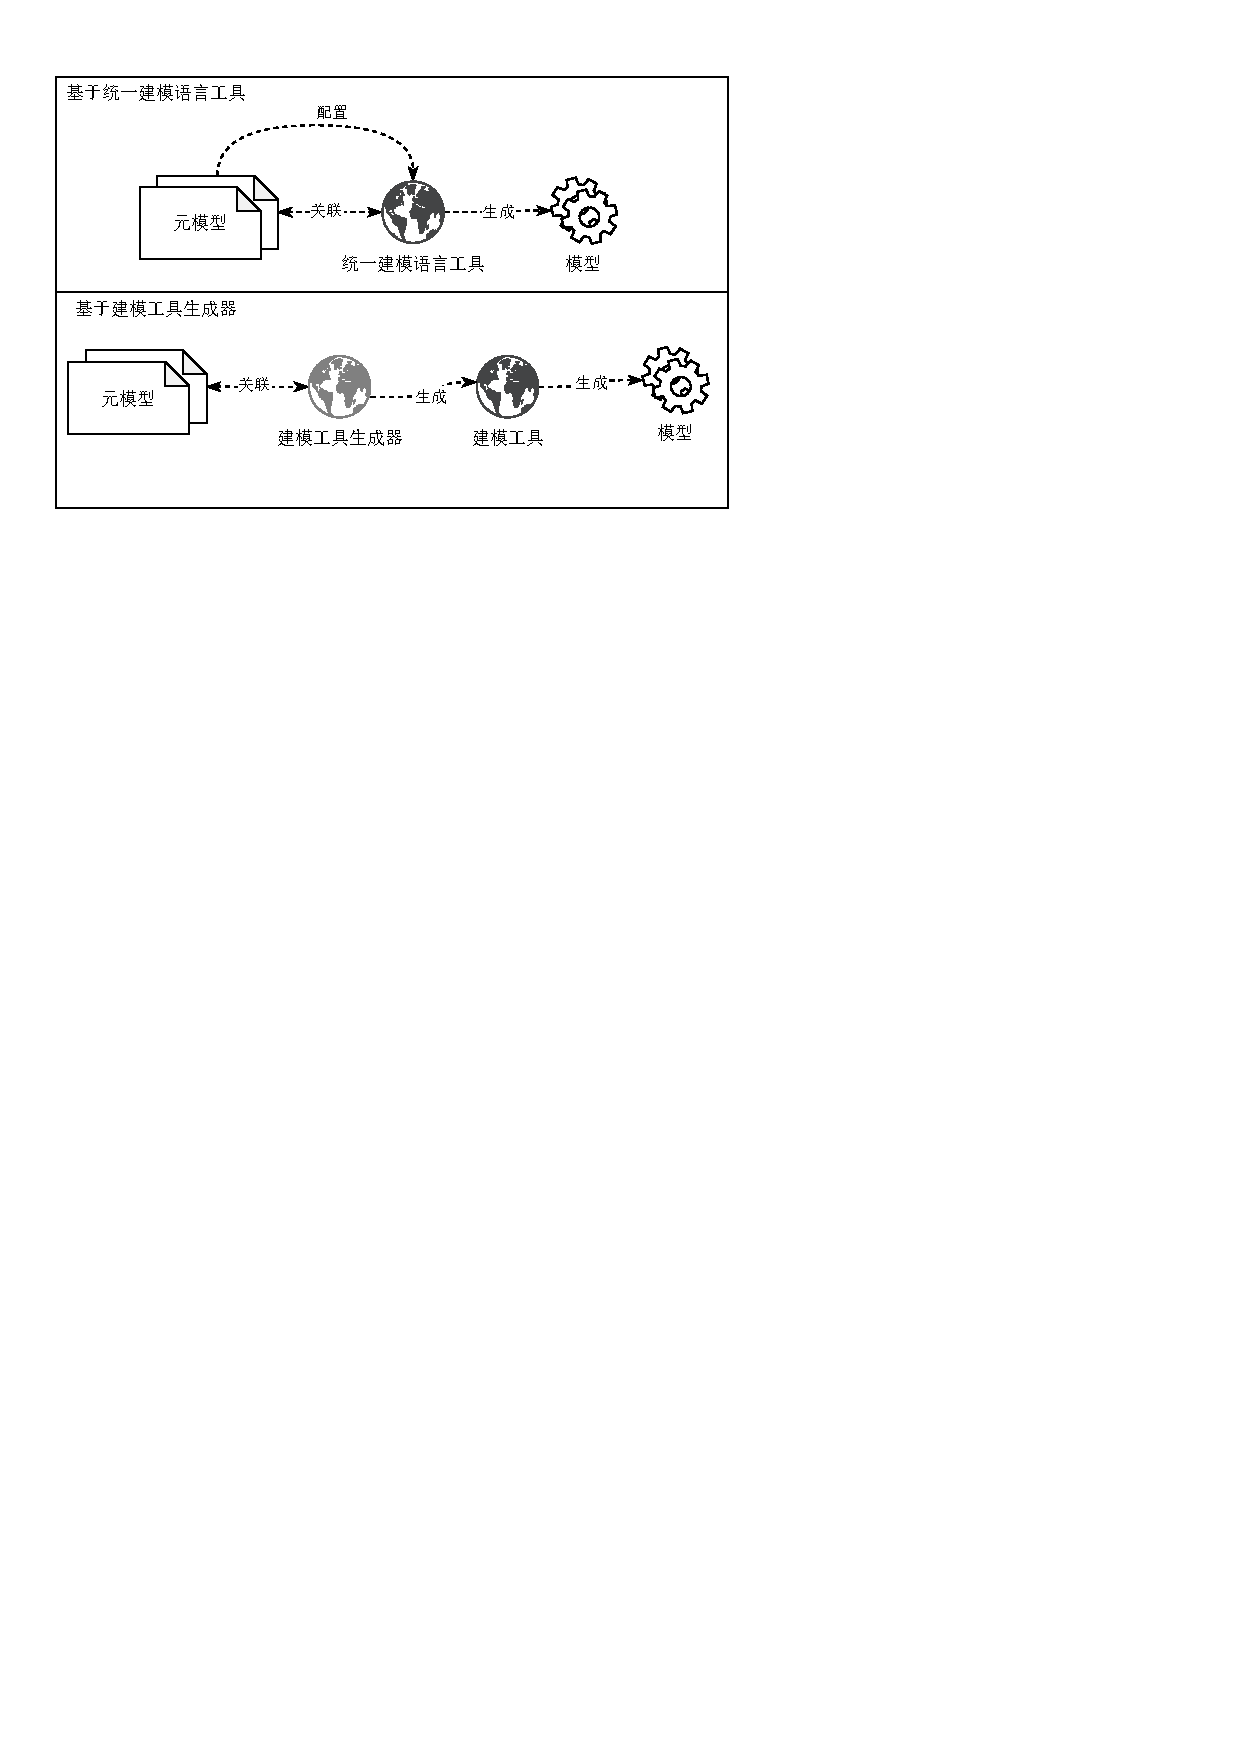
\includegraphics[width=0.8\textwidth]{FIGs/chapter3/2kindsmodeling.pdf} %中括号中的参数是设置图片充满文档的大小,你也可以使用小数来缩小图片的尺寸。
    \caption{两种建模工具实施方式} %caption是用来给图片加上图题的
    \label{2kindsmodeling} %这是添加标签,方便在文章中引用图片。
\end{figure}%figure环境

4)验证。针对最终形成的特定领域建模语言,还可以进行使用效果的验证。包含定性和定量的分析方法,
定性分析主要关注建模语言使用者的感受,从易用性、可靠性以及正确性等方面进行考察;
定量分析主要关注使用新建模语言的效率,从建模各阶段耗费时间进行统计分析\cite{kardas2018domain}。


\section{建模支持工具实现技术}

本小节将对建模支持工具实现技术进行介绍。
本文实现的建模支持工具所需技术包括可视化建模展示所用的mxGraph,
前端界面构建所用的Vue.js和ElementUI;
后端服务器所需技术包括Spring Boot和ElasticSearch。


\textbf{mxGraph}

mxGraph\footnotemark[5]\footnotetext[5]{mxGraph项目地址:https://github.com/jgraph/mxgraph}
是一个使用SVG和HTML进行渲染的JavaScript图表库客户端,
支持交互式图形和图表的快速创建,在主流的浏览器中都能良好运行。
支持在网页中设计和编辑工作流图、流程图、网络图和各种图表。
mxGraph库不使用任何第三方软件,不需要任何插件,并且可以集成在几乎任何框架中。
mxGraph拥有完善的绘图功能,许多大型产品底层都使用其进行绘图和渲染。
不仅拥有JavaScript源码版本,还有Java源码版本,拥有便于移植和适配性强等特点,
还支持以XML或图片形式进行展示等功能。
本文使用mxGraph作为可视化建模的支持技术,通过在网页中运行mxGraph,
来达到拖拽绘制模型、点击连线、双击修改文字以及导出建模结果等功能。

\textbf{Vue.js}

Vue.js\footnotemark[6]\footnotetext[6]{Vue 官网https://cn.vuejs.org/}是一套用于构建用户界面的渐进式框架。
与其它大型框架不同,Vue.js可以自底向上逐层应用。
Vue.js的核心库只关注视图层,能方便地获取数据更新,并通过组件内部特定的方法实现视图与模型的交互。
此外,Vue.js容易上手,与第三方库或现有项目进行整合时方便,
与主流的开发工具链以及各种支持类库结合使用时,Vue.js也完全能够为复杂的单页应用提供驱动。
得益于响应式设计,Vue.js获取数据更新十分方便。
响应式是指MVC模型中的视图随着模型变化而变化。
在Vue.js中,开发者只需将视图与对应的模型进行绑定,Vue.js便能自动观测模型的变动,并重绘视图,
这一特性使得Vue.js的状态管理变得相当简单直观。
Vue.js构建的界面简洁美观,交互方式易于理解,交互响应速度快,本文使用Vue.js来实现前端的用户界面展示与交互。

组件(Componet)也是Vue.js的一大基础功能。组件可以被复用,封装可多次重用的代码逻辑,
复用的组件能更加方便地进行管理、修改和优化。
组件还可以以不同形式(如数组、树)组织起来,几乎任意类型的应用的界面都可以抽象为一个组件树,
从而构建出大型复杂的应用。

如图\ref{vue}所示描述了响应式设计追踪变化的过程。
当一个普通的JavaScript对象传入Vue实例作为data选项时,
Vue将遍历此对象所有的property,并使用Object.defineProperty把这些property全部转为getter/setter。
这些getter/setter对用户来说是不可见的,但是在内部它们让Vue能够追踪依赖,在property被访问和修改时通知变更。
每个组件实例都对应一个watcher实例,它会在组件渲染的过程中把“接触”过的数据property记录为依赖。
之后当依赖项的setter触发时,会通知watcher,从而使它关联的组件重新渲染。

\begin{figure}[h] %figure环境,h默认参数是可以浮动,不是固定在当前位置。如果要不浮动,你就可以使用大写float宏包的H参数,固定图片在当前位置,禁止浮动。
    \centering %使图片居中显示
    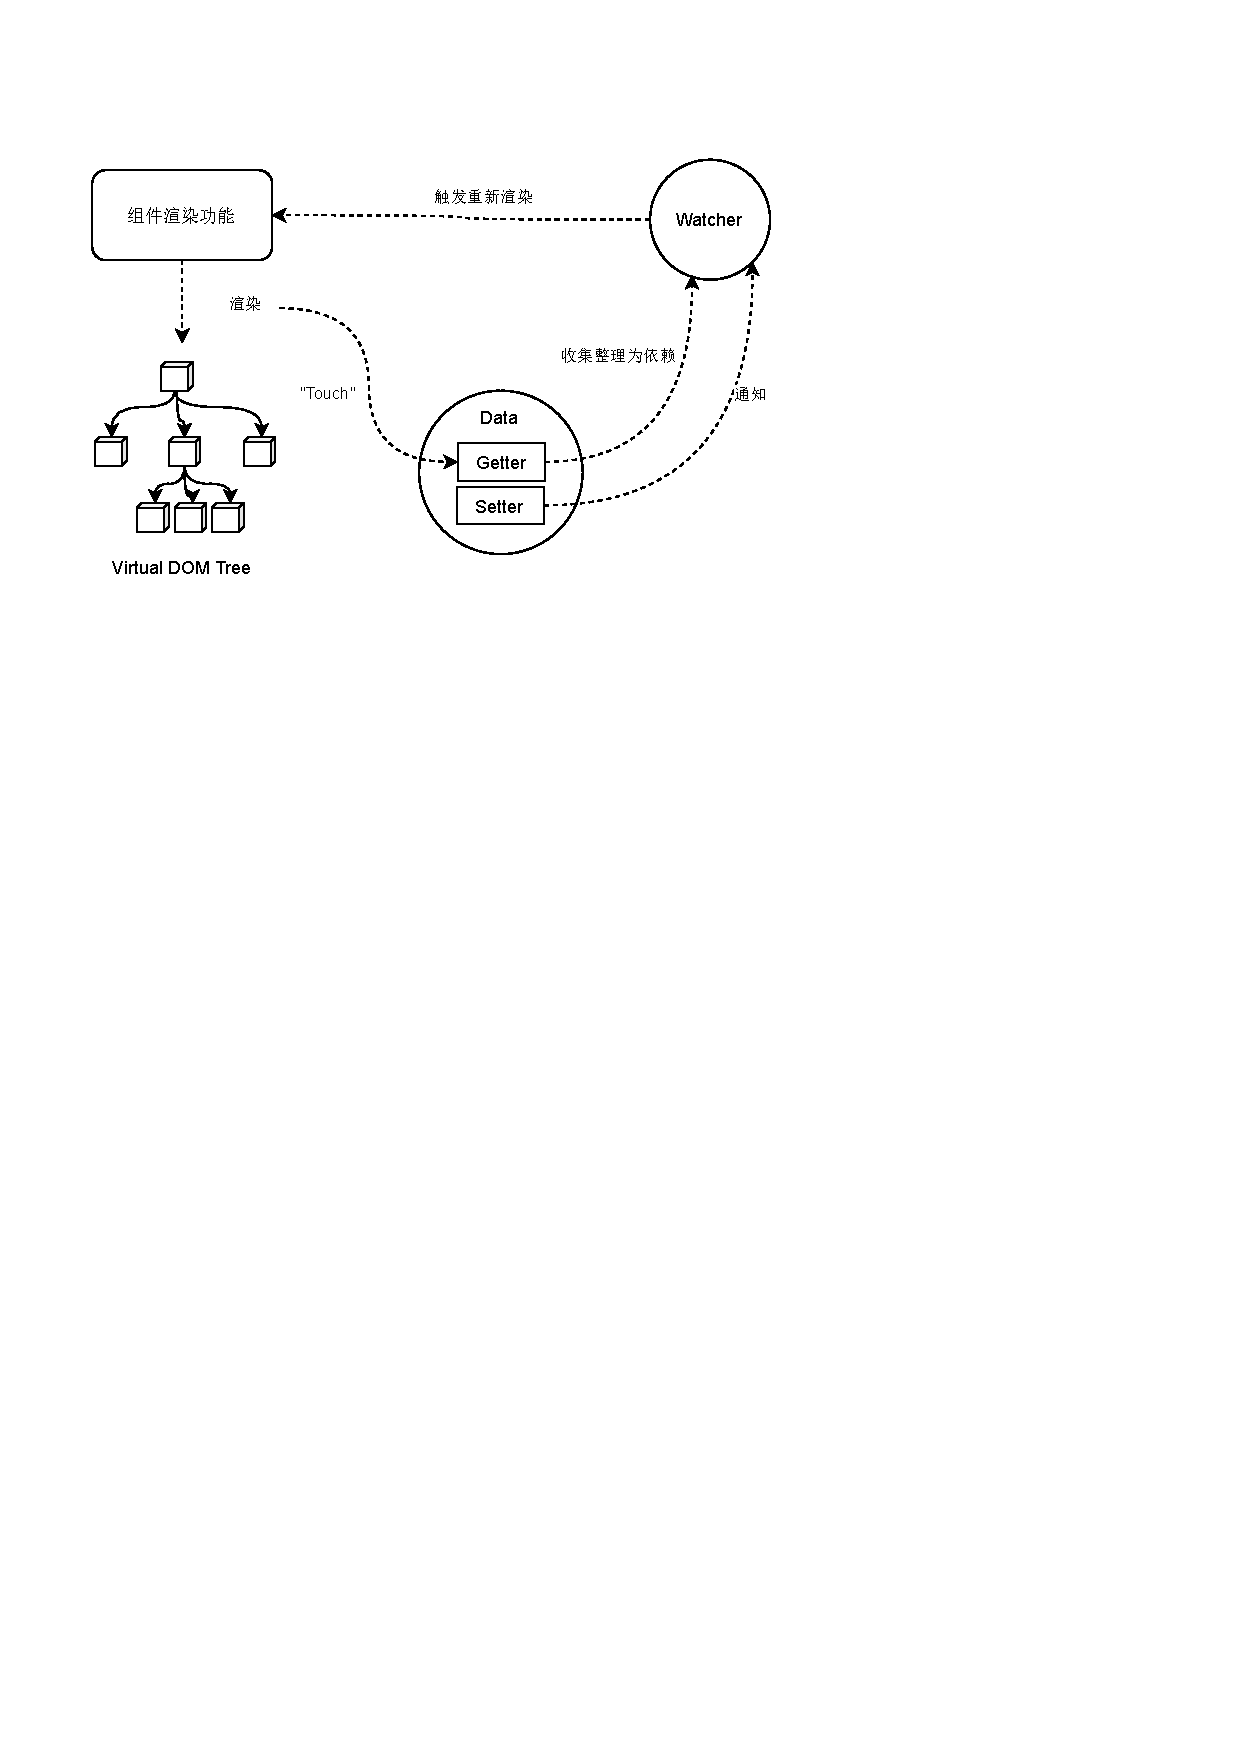
\includegraphics[width=0.8\textwidth]{FIGs/chapter2/vue.pdf} %中括号中的参数是设置图片充满文档的大小,你也可以使用小数来缩小图片的尺寸。
    \caption{响应式设计追踪变化} %caption是用来给图片加上图题的
    \label{vue} %这是添加标签,方便在文章中引用图片。
\end{figure}%figure环境

\textbf{ElementUI}

ElementUI\footnotemark[7]\footnotetext[7]{ElementUI主页:https://element.eleme.io}
是一套基于Vue2.0的桌面端组件库,包含了大量的页面设计组件与资源,
秉承了一致、反馈、效率、可控的设计原则,帮助使用者快速搭建网站前端交互界面。
ElementUI强调界面元素一致及用户界面和生活场景一致,做到清晰的页面反馈和控制反馈,
提供的组件表述清晰直白,使用方式简单高效,用户可以自由准确地使用这些组件进行自主性操作。
本文使用ElementUI对前端组件进行统一管理,对数据和组件进行绑定和交互。

\textbf{Spring Boot}

Spring Boot\footnotemark[8]\footnotetext[8]{SpringBoot主页:https://spring.io/projects/spring-boot}
是为了简化Spring应用搭建以及开发过程的一种框架。
Spring Boot提供起步依赖和自动依赖管理,
以注解形式进行配置,
代替了不易阅读的XML格式配置文件。
集成的Web服务器不需要再次对网络请求进行复杂处理,可以快速构建后端服务器。
本文使用Spring Boot开发后端服务,以服务器形式为前端提供接口服务。

\textbf{ElasticSearch}

ElasticSearch\footnotemark[9]\footnotetext[9]{ElasticSearch主页:https://www.elastic.co/cn/}
是一个基于Lucene\cite{bialecki2012apache}库的搜索引擎。
ElasticSearch可以用于搜索各种文档,具有接近实时的搜索效果,可以通过JSON和Java API提供服务,
适合含有大量数据的文档搜索与存储。本文项目中的模型结果以文档形式存储在ElasticSearch中,
能够支持快速检索。

\section{本章小结}

本章主要介绍了与本文工作相关的理论与支持技术。
首先对领域驱动设计中的重要概念进行解释,主要介绍了战术建模包括的重要模式和一些相关概念;
然后对建模语言进行了介绍,
重点解释了元模型,UML profile机制以及OCL等支持构建建模语言的方式;
还介绍了构建特定领域建模语言的方法和具体过程;
最后,介绍了支持工具需要用到的技术,
包括可视化技术mxGraph,前端支持工具Vue.js和ElementUI,以及后端技术Spring Boot和ElasticSearch。





